\subsection{Absolute Pilot Outcomes and Concentration}
This additional interpretation is exploratory. In hierarchical scheduling, the single condition has accuracy 81.25\%, versus 94.79\% with exact repetition. Each arm has 96 trajectories from 12 independent bases, pooling both worlds, two policies and two stochastic repetitions. Matched outcomes comprise 14 improvements, 1 regression and 81 unchanged outcomes. No contract failures or truncations explain this difference.
Six bases improve on average, one regresses and five have zero net change. One base accounts for seven improved cells. Excluding it reduces the gain to 6.82 percentage points; the full leave-one-base-out range is 6.82--15.91 points. These omissions are descriptive, not additional significance tests.
Figure~\ref{fig:absolute-pilot} shows absolute accuracy and paired effects. Table~\ref{tab:paired-world-detail} requires correct decisions in both worlds. Figure~\ref{fig:failure-locations} distinguishes observable failure locations.
\begin{figure}[tb]\centering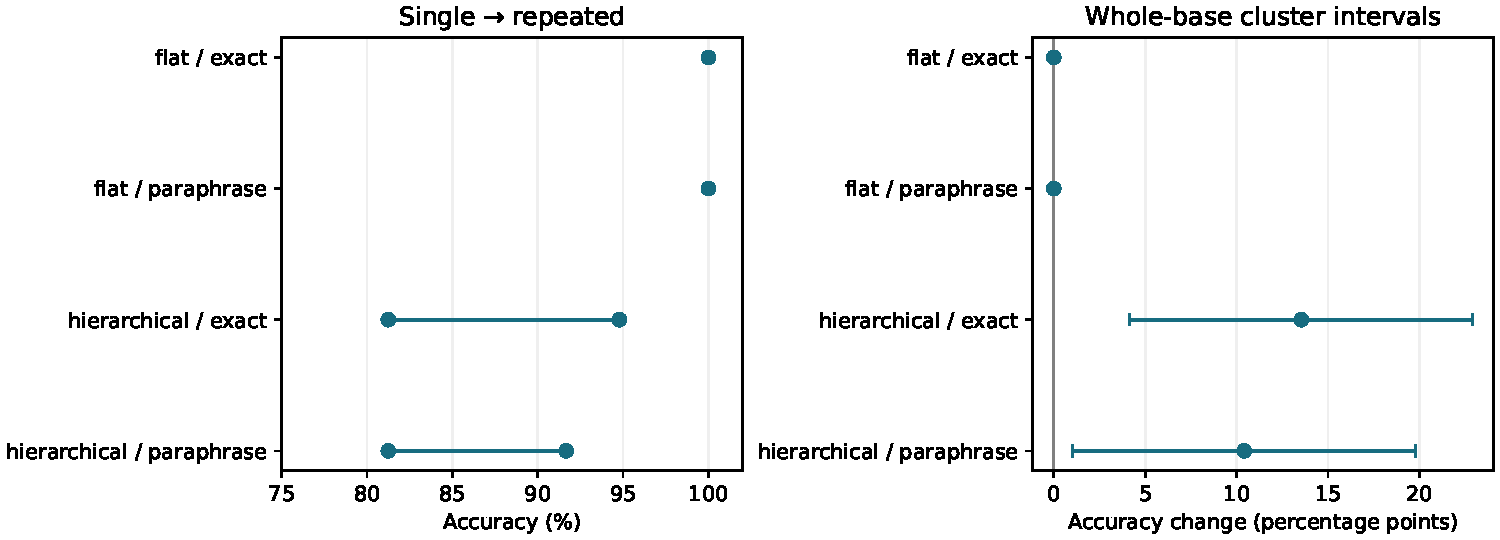
\includegraphics[width=\textwidth]{../results/pilot-interpretation-v2/figures/absolute-and-paired-effects.pdf}\caption{Pilot scheduling accuracy and paired repetition effects.}\label{fig:absolute-pilot}\end{figure}
\begin{table}[tb]\centering\small\caption{Both paired-world answers correct; scheduling hierarchy.}\label{tab:paired-world-detail}
\begin{tabular}{llrrr}\toprule Edit & Repeat & Single (\%) & Repeated (\%) & Difference [95\% CI]\\\midrule
Harmless & Exact & 79.17 & 95.83 & 16.67 [0.00, 33.33]\\
Harmless & Paraphrase & 79.17 & 91.67 & 12.50 [-8.33, 33.33]\\
Consequential & Exact & 66.67 & 87.50 & 20.83 [8.33, 33.33]\\
Consequential & Paraphrase & 66.67 & 79.17 & 12.50 [8.33, 16.67]\\
\bottomrule\end{tabular}\end{table}
Each paired-world row uses six bases and 24 matched world-pair cells per arm. Success requires both correct answers. Merely changing or retaining a choice does not count. Intervals resample bases within family and edit-status strata.
\begin{figure}[tb]\centering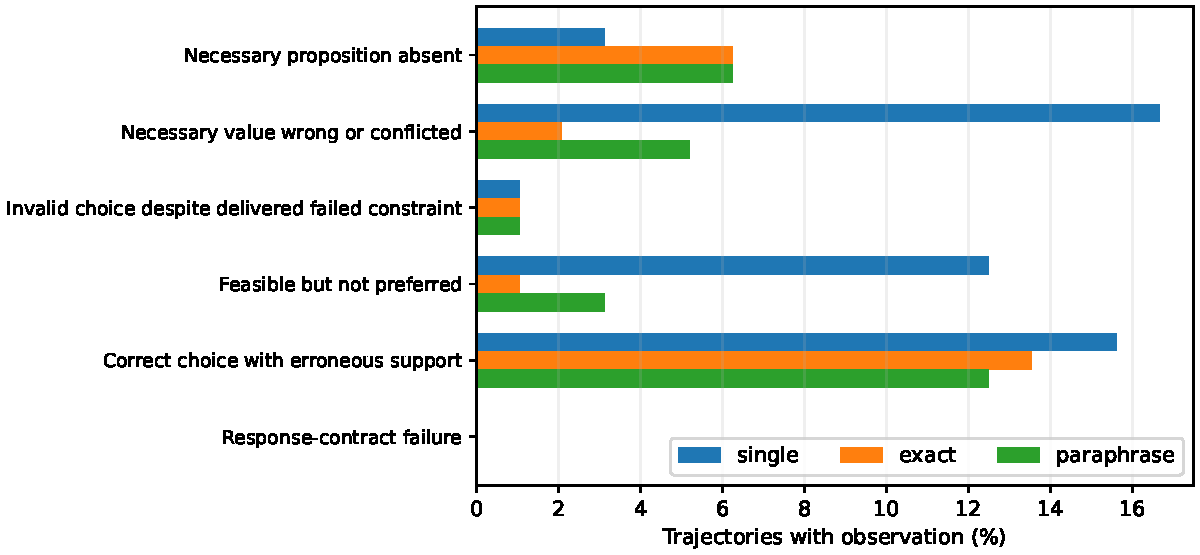
\includegraphics[width=\textwidth]{../results/pilot-interpretation-v2/figures/observable-failure-locations.pdf}\caption{Observable pilot failures; labels overlap.}\label{fig:failure-locations}\end{figure}
Keyed assertions bind the full public scope, including entity, units, condition, criterion and version. Numerical preservation at another key does not count. These deterministic labels describe messages and choices; they do not identify internal reasoning or causal mediation. Correct final choices can coexist with incorrect supporting assertions. The extension section reports completion status for the transport and root-only interventions.
